\section{Лекция 7 (20.10)}

\subsection{Инициализация решения}
\label{sec:ns2d-init}

Схема решения SIMPLE является итерационной, а значит для начала расчётов ей требуется
какое-то начальное приближение параметров, описывающих течение.
Для решения задачи в каверне мы использовали нулевое приближение ($u=v=p=0$).
Однако, при расчёте открытых течений, такое приближение не является оптимальным,
потому что не соответствует входным граничным условиям.
В таких задачах удобно в качестве начального приближения использовать потенциальное решение.

\subsubsection{Задача о потенциале течения}
Введем потенциал $\phi$ векторного поля скорости как $\vec{u} = \nabla\phi$.
В двумерной декартовой системе координат получим
\begin{equation}
\label{eq:potential2}
\begin{array}{l}
	u = \ddfr{\phi}{x}, \\[10pt]
	v = \ddfr{\phi}{y}. \\[10pt]
\end{array}
\end{equation}

Для модели несжимаемой жидкости из уравнения неразрывности \cref{eq:ns2d_div}
получим уравнение для потенциала
\begin{equation}
	\label{eq:potential2_eq}
	\dfrq{\phi}{x} + \dfrq{\phi}{y} = 0.
\end{equation}

В качестве  граничных условиях на всех непротекаемых поверхностях используем условие
$v_n = 0$:
\begin{equation}
	\label{eq:potential2_bcwall}
	\left. \dfr{\phi}{n} \right|_{wall} = 0
\end{equation}

Во входном и выходном сечениях используем условие постоянной нормальной скорости $v_n$,
вычисляемой из известного расхода $Q$:
\begin{equation}
	\label{eq:potential2_bcio}
	\left. \dfr{\phi}{n} \right|_{io} = v_n = Q/\left|\Gamma_{io}\right|.
\end{equation}

После решения задачи \cref{eq:potential2_eq,eq:potential2_bcwall,eq:potential2_bcio}
компонеты скорости находятся прямым дифференцированием по формулам \cref{eq:potential2}.

\subsubsection{Аппроксимация на разнесённой сетке}
Исходя из необходимости вычислять выражения \cref{eq:potential2},
значение потенциала удобно аппроксимировать в ``чёрных'' узлах сетки (\figref{fig:staggered_grid}).

Тогда сеточное уравнение для узла $i+\tfrac12, j+\tfrac12$ для выражения \cref{eq:potential2_eq}
будет записано в виде
\begin{equation}
\label{eq:potential2_slae}
\frac{-\phi_{i-\tfrac12, j+\tfrac12} + 2 \phi_{i+\tfrac12, j+\tfrac12} - \phi_{i+\tfrac32,j+\tfrac12}}{h_x^2}
+
\frac{-\phi_{i+\tfrac12, j-\tfrac12} + 2 \phi_{i+\tfrac12, j+\tfrac12} - \phi_{i+\tfrac12,j+\tfrac32}}{h_y^2}
= 0.
\end{equation}

Граничные условия \cref{eq:potential2_bcwall}, \cref{eq:potential2_bcio}
используются для вычисления значений в фиктивных узлах сетки.

Так, пусть левая граница $i=0$ есть входная граница течения. Тогда
\begin{equation*}
\left. \dfr{\phi}{n} \right|_{left} = \left. -\dfr{\phi}{x} \right|_{left} = \frac{\phi_{-\tfrac12, j+\tfrac12} - \phi_{\tfrac12, j+\tfrac12}}{h_x} = v_n.
\end{equation*}
Отсюда получим
\begin{equation*}
\phi_{-\tfrac12, j+\tfrac12} = h_x v_n + \phi_{\tfrac12, j+\tfrac12}.
\end{equation*}

Поэтому уравнение \cref{eq:potential2_slae} для левых узлов сетки примет вид
\begin{equation*}
\frac{\phi_{\tfrac12, j+\tfrac12} - \phi_{\tfrac32,j+\tfrac12}}{h_x^2}
+
\frac{-\phi_{\tfrac12, j-\tfrac12} + 2 \phi_{\tfrac12, j+\tfrac12} - \phi_{\tfrac12,j+\tfrac32}}{h_y^2}
= \frac{v_n}{h_x}.
\end{equation*}

Если нижняя граница сетки $j=0$ непротекаемая, то условие \cref{eq:potential2_bcwall} даёт
\begin{equation*}
\phi_{i+\tfrac12, -\tfrac12} = \phi_{i+\tfrac12, \tfrac12}
\end{equation*}
и уравнение \cref{eq:potential2_slae} запишется как
\begin{equation*}
\frac{-\phi_{i-\tfrac12, j+\tfrac12} + 2 \phi_{i+\tfrac12, j+\tfrac12} - \phi_{i+\tfrac32,j+\tfrac12}}{h_x^2}
+
\frac{\phi_{i+\tfrac12, \tfrac12} - \phi_{i+\tfrac12,\tfrac32}}{h_y^2}
= 0.
\end{equation*}

Поскольку задача в задаче для потенциала
используются только граничные условия второго рода,
то для получения однозначного решения необходимо
явно указать значение в одном из узлов. Например
\begin{equation*}
\phi_{\tfrac12, \tfrac12} = 0.
\end{equation*}

После вычисления сеточного вектора $\{\phi\}$
значения компонент скорости получаются из формул \cref{eq:potential2}:
\begin{align*}
	&u_{i, j+\tfrac12} = \frac{\phi_{i+\tfrac12, j+\tfrac12} - \phi_{i-\tfrac12, j+\tfrac12}}{h_x}\\
	&u_{0, j+\tfrac12} = v_n
\end{align*}

\subsection{Конвективный теплообмен}
\subsubsection{Уравнение теплопроводности}

Дополним нестационарную систему уравнений течения \cref{eq:ns2d_nonstat} уравнением теплообмена
\begin{equation*}
\rho c_p\left(\dfr{T}{t} + u\dfr{T}{x} + v\dfr{T}{y}\right) = \lambda\left(\dfrq{T}{x} + \dfrq{T}{y}\right).
\end{equation*}
Здесь $T$ -- температура течения, К; $\rho$ -- плотность жидкости, кг/м$^3$; $c_p$ -- теплоёмкость, Дж/кг/К;
$\lambda$ -- теплопроводность, Вт/м/К.

В безразмерном виде это уравнение примет вид
\begin{equation}
\label{eq:ns2d_nonstat_temperature}
\dfr{T}{t} + u\dfr{T}{x} + v\dfr{T}{y} = \frac{1}{\Pen}\left(\dfrq{T}{x} + \dfrq{T}{y}\right).
\end{equation}
где безразмерная температура $T$ вычислена через размерную $T^{dim}$ как 
$$
T = \frac{T^{dim} - T^0}{\triangle T},
$$
а число Пекле $\Pen$ есть
$$
\Pen = \frac{U L}{a}, \quad a = \frac{\lambda}{\rho c_p}.
$$

\subsubsection{Дискретизация по времени}

Пользуясь обозначениями из п. \ref{sec:simple-nonstat-algo}
запишем неявную дискретизацию по времени уравнения \cref{eq:ns2d_nonstat_temperature} в виде

\begin{equation}
\label{eq:ns2d_nonstat_temperature_semi}
\frac{\hat T - \check T}{\dt} + \hat u\dfr{\hat T}{x} + \hat v\dfr{\hat T}{y} = \frac{1}{\Pen}\left(\dfrq{\hat T}{x} + \dfrq{\hat T}{y}\right).
\end{equation}

Полученное уравнение не содержит значений $u, v$ с текущего итерационного слоя,
и значит может быть решено один раз в конце шага по времени, когда сходимость уже достигнута.

\subsubsection{Аппроксимация на разнесённой сетке}

Пространственную аппроксимацию уравнения \cref{eq:ns2d_nonstat_temperature_semi}
будем проводить на разнесённой сетке в центральных (``чёрных'') узлах сетки (\figref{fig:staggered_grid}).
При этом конвективную производную будем приближать с помощью симметричной разности.
Полученная конечная разность для узла $i+\tfrac12, j+\tfrac12$ примет вид
\begin{align}
\label{eq:ns2d_nonstat_temperature_scheme}
\frac{1}{\dt}\hat T_{i+\tfrac12,j+\tfrac12}
    & + \hat u_{i+\tfrac12, j+\tfrac12}\frac{\hat T_{i+\tfrac32, j+\tfrac12} - \hat T_{i-\tfrac12, j+\tfrac12}}{2h_x}\\
    \nonumber
    & + \hat v_{i+\tfrac12, j+\tfrac12}\frac{\hat T_{i+\tfrac12, j+\tfrac32} - \hat T_{i+\tfrac12, j-\tfrac12}}{2h_y}\\
    \nonumber
    & + \frac{1}{\Pen} \frac{-\hat T_{i+\tfrac32, j+\tfrac12} + 2\hat T_{i+\tfrac12,j+\tfrac12} - \hat T_{i-\tfrac12, j+\tfrac12}}{h_x^2} \\
    \nonumber
    & + \frac{1}{\Pen} \frac{-\hat T_{i+\tfrac12, j+\tfrac32} + 2\hat T_{i+\tfrac12,j+\tfrac12} - \hat T_{i+\tfrac12, j=\tfrac12}}{h_x^2} \\
    \nonumber
    & = \frac{1}{\dt}\check T_{i+\tfrac12,j+\tfrac12}.
\end{align}

Значения компонент скорости в центрах ячеек вычисляются с помощью ближайщей полусуммы
\begin{align*}
&\hat u_{i+\tfrac12, j+\tfrac12} \approx \frac{\hat u_{i, j+\tfrac12} + \hat u_{i+1, j+\tfrac12}}{2}, \\
&\hat v_{i+\tfrac12, j+\tfrac12} \approx \frac{\hat v_{i+\tfrac12, j} + \hat v_{i+\tfrac12, j+1}}{2}.
\end{align*}


\subsubsection{Граничные условия}

Учёт граничных условий производится за счёт вычисления значений в фиктивных узлах около границ.

Пусть требуется учесть условие на левой стенке ($i=0$).
Тогда соответствующий фиктивный узел будет иметь индекс $-\tfrac12, j$.
Ниже приведём его выражения для трёх типов граничных условий.

\subsubsubsection{Условия первого рода}
Пусть
\begin{equation}
\label{eq:ns2d_temperature_bc1}
\left. T\right|_{left} = T^{\Gamma}
\end{equation}
Тогда
$$
\frac{T_{-\tfrac12, j+\tfrac12} + T_{\tfrac12, j+\tfrac12}}{2} = T^{\Gamma}.
$$
Отсюда 
$$
T_{-\tfrac12, j+\tfrac12} = -T_{\tfrac12, j+\tfrac12} + 2 T^{\Gamma}.
$$
Таким образом, если в матрицу $A^T$ левой части выражения \cref{eq:ns2d_nonstat_temperature_scheme}
в фиктивную колонку $k\left[-\tfrac12, j+\tfrac12\right]$ требуется добавить
какое-то значение $a$, это равносильно добавлению этого выражнеия с обратным знаком в диагональ
и удвоенного выражения, умноженного на граничное значение, в правую часть $b^T$:
\begin{align}
\nonumber
&k_0 = k\left[\tfrac12, j + \tfrac12\right], \quad k_1 = k\left[-\tfrac12, j + \tfrac12\right], \\
\label{eq:ns2d_temperature_bc1_scheme}
&A^T_{k_0, k_1} {{+}{=}} a \hence
     A^T_{k_0, k_0} \minuseq a, \quad b^T_{k_0} \minuseq 2 a T^\Gamma.
\end{align}


\subsubsubsection{Условия второго рода}
Если на левой границе задано условие второго рода
\begin{equation}
\label{eq:ns2d_temperature_bc2}
\left.\dfr{T}{n}\right|_{left} = -\left. \dfr{T}{x} \right|_{left} = q
\end{equation}
То вычисление фиктивного узла производится из конечной разности вида
$$
\frac{T_{-\tfrac12, j+\tfrac12} - T_{\tfrac12, j+\tfrac12}}{h_x} = q.
$$
Отсюда 
$$
T_{-\tfrac12, j+\tfrac12} = T_{\tfrac12, j+\tfrac12} + h_x q
$$
Тогда
\begin{align}
\label{eq:ns2d_temperature_bc2_scheme}
&A^T_{k_0, k_1} {{+}{=}} a \hence
     A^T_{k_0, k_0} \pluseq a, \quad b^T_{k_0} \minuseq h_x q
\end{align}

\subsubsubsection{Условия третьего рода}
Пусть на левой границе задано условие второго рода
\begin{equation}
\label{eq:ns2d_temperature_bc3}
\left.\dfr{T}{n}\right|_{left} = -\left. \dfr{T}{x} \right|_{left} = \alpha T + \beta
\end{equation}

Расписывая производную и вычисляя значение температуры на стенке через полусумму, получим
$$
\frac{T_{-\tfrac12, j+\tfrac12} - T_{\tfrac12, j+\tfrac12}}{h_x} = \alpha \frac{T_{-\tfrac12, j+\tfrac12} + T_{\tfrac12, j+\tfrac12}}{2} + \beta.
$$
Отсюда выразим значение в фиктивном узле
$$
T_{-\tfrac12, j+\tfrac12} = \frac{2 + \alpha h_x}{2-\alpha h_x} T_{\tfrac12, j+\tfrac12} + \frac{2\beta h_x}{2 - \alpha h_x}
$$
Тогда
\begin{align}
\label{eq:ns2d_temperature_bc3_scheme}
&A^T_{k_0, k_1} {{+}{=}} a \hence
     A^T_{k_0, k_0} \pluseq \frac{2 + \alpha h_x}{2 - \alpha h_x} a, \quad b^T_{k_0} \minuseq \frac{2 \beta h_x}{2 - \alpha h_x} a.
\end{align}

\subsubsubsection{Универсальность условий третьего рода}
Условие третьего рода \cref{eq:ns2d_temperature_bc3} можно использовать для моделирования условий первого и второго рода.
Так, условия второго рода \cref{eq:ns2d_temperature_bc2} получаются, если положить $\alpha = 0$, $\beta = q$.
А условия первого \cref{eq:ns2d_temperature_bc1}, -- если $\alpha = \eps^{-1}, \beta = -\eps^{-1}T^\Gamma$, где $\eps$ -- малое положительное число.

Если подставить эти выражения в формулу \cref{eq:ns2d_temperature_bc3_scheme}, то можно убедится,
что они дадут выражения \cref{eq:ns2d_temperature_bc2_scheme} и \cref{eq:ns2d_temperature_bc1_scheme} (в пределе при $\eps \to 0$)
соответственно.

\subsubsection{Коэффициент теплообмена}
На границах, где заданы условия первого рода \cref{eq:ns2d_temperature_bc1}
можно вычислить тепловой поток, тем самым
определив, сколько тепловой энергии требуется для
поддержания этой постоянной температуры.

Безразмерный интегральный коэффициент теплообмена (интегральное число Нуссельта) определяется как
\begin{equation}
\label{eq:integral_nu}
\Nun = \arint{\dfr{T}{n}}{\gamma}{s}.
\end{equation}

Для получения размерной мощности из этого безразмерного коэффициента (измеряемой в Ваттах),
необходимо умножить его на $\lambda \triangle T L$.

Вычисление интегрального числа Нуссельта из определения \cref{eq:integral_nu} происходит по той
же схеме, что и вычисление коэффициентов сил \cref{eq:ns2d_gamma_quadrature}.
При этом нормальная производная на границе $\dsfr{T}{n}$ вычисляется в виде
\begin{equation}
\label{eq:dtdn_scheme}
(x,y)\in\gamma_i: \quad \dfr{T}{n} \approx \frac{T^\Gamma - T_k}{h/2},
\end{equation}
где $\gamma_i$ -- отрезок границы, $k$ -- индекс ячейки, прилегающей к этому отрезку,
$h$ -- шаг сетки, поперёк границы ($h_x$ для вертикальных границ и $h_y$ -- для горизонтальных).

\subsection{Тестовые примеры}
\clisting{open}{"test/linear_2d_simple_test.cpp"}

\subsubsection{Задача о равномерном течении}
Рассмотрим задачу о стационарном прямолинейном течении с граничными условиями
\begin{align*}
(x,y)\in\Gamma_{in}:      \quad & u=1, v=0, \\
(x,y)\in\Gamma_{top,bot}: \quad & \dfr{u}{n} = 0, v = 0, \\
(x,y)\in\Gamma_{out}:     \quad & u\dfr{u}{x} = 0, v = 0.
\end{align*}
Очевидно, что точным решением этой задачи будут $u=1, v=0, p=0$.
В случае использования алгоритма инициализации (п. \ref{sec:ns2d-init}) 
мы бы сразу получили этот ответ. Но здесь в качестве теста будем начинать итерации
из состояния покоя $u=v=p=0$.

Задача решается в области $[0, 2]\times[-\tfrac12, \tfrac12]$
c использованием алгоритма SIMPLEC c $E=4$ и разбиением на единицу длины $n_{un} = 20$.

Программа реализована в тесте \ename{linear2-simple} в файле \ename{linear_2d_simple_test.cpp}.

Программа по расчёту этой задачи отличается от рассмотренной ранее задачи
в каверне (п. \ref{sec:prog-cavern2}) только наличием условий
входного и выходного сечений.

\paragraph{Шаг алгоритма SIMPLE}
В функции \cvar{step()}, описывающей основной шаг алгоритма SIMPLE,
добавлено вычисление граничных значений поправки скорости $u'$ из \cref{eq:ns2d_ustroke_from_balance}
необходимых для соблюдения баланса массы (\cvar{compute_u_stroke_outflow}).
\clisting{block}{"double Linear2DSimpleWorker::step()"}
В дальнейшем эти условия используются для расчёта поправки давления
и для расчёта самой поправки скорости. 

\subsubsubsection{Учёт граничных условий}
\paragraph{Вычисление поправки скорости на выходной границе}
Функция \cvar{compute_u_stroke_outflow}, реализующая вычисление формулы \cref{eq:ns2d_ustroke_from_balance},
имеет вид
\clisting{block}{"std::vector<double> Linear2DSimpleWorker::compute_u_stroke_outflow"}.
Здесь в цикле по вертикальным граням вычисляются расходы по входному и выходному сечениям
(\cvar{qin}, \cvar{qout}),
далее находится поправка скорости (\cvar{diff_u}), постоянная для всех выходных отрезков,
и возвращается вектор, содержащий эту поправку для всех выходных отрезков.

\paragraph{Учёт гранииных условий для $u^*$}
\clisting{to-start}{}
Для учёта граничных условий входа и выхода при сборке уравнения для $u^*$ в функции \cvar{assemble_u_slae}
используется цикл
\clisting{pass}{"void Linear2DSimpleWorker::assemble_u_slae()"}
\clisting{block}{"for (size_t j=0; j< _grid.ny(); ++j)"}
Здесь для левой границы
согласно \cref{eq:ns2d_au_bc_left}
жёстко устанавливается единичное значение.
А для правой границы используются соотношения \cref{eq:ns2d_outflow_ustar_mat}.

\paragraph{Учёт граничных условий для p'}

Найденные поправки скорости на выходной границе
должны быть учтены при решении задачи для $p'$ согласно
\cref{eq:ns2d_outflow_pstrike_mat}
Сборка матрицы левой части при этом останется неизменной.
Действительно, распишем производную на правой (выходной) границе
$$
d^u\dfr{p'}{x}_{n_x, j+\tfrac12} \approx d^u\frac{p'_{k_1} - p'_{k_0}}{h_x}
$$
входящую в выражение \cref{eq:ns2d_d2pdx2}.
Где $k_0 = k[n_x - \tfrac12, j+\tfrac12]$ -- реальный,
а $k_1 = k[n_x + \tfrac12, j+\tfrac12]$ -- находящийся правее него фиктивный узлы сетки.
Наличие этой производной требует добавления
выражения $d^u/h_x^2$ в реальный (диагональный) столбец $k_0$
и выражения $-d^u/h_x^2$ в фиктивный столбец $k_1$ матрицы $A^p$ в строке $k_0$.
Следуя алгоритму \cref{eq:ns2d_outflow_pstrike_mat} добавление
значения в фиктивный столбец равносильно добавлению этого же значения в диагональный столбец.
То есть два этих значения взаимоуничтожаться. Останется только модифицировать столбец правых членов.
Альтернативно можно просто подставить значение производной 
\cref{eq:ns2d_outflow_pstroke} в дисретизованное выражение 
\cref{eq:ns2d_d2pdx2}, и, поскольку оно не содержит в себе $p'$, унести его в правую часть
с обратным знаком и делением на $h_x$.

Учёт граничных условий в правой части осуществляется в функции
\cvar{assemble_p_stroke_solver} за счёт модификации правой части для узлов,
расположенных около выходной границы:
\clisting{to-start}{}
\clisting{pass}{"void Linear2DSimpleWorker::assemble_p_stroke_solver()"}
\clisting{block}{"// outflow compensation"}

\paragraph{Учёт граничных условий для $u'$}
Явным образом предварительно найденные
граничные значения для поправки скорости присваиваются в фукнции
\cvar{"compute_u_stroke"}:
\clisting{to-start}{}
\clisting{pass}{"std::vector<double> Linear2DSimpleWorker::compute_u_stroke"}
\clisting{block}{"// outflow"}

\subsubsubsection{Анализ результатов}
До невязки $\eps=10^{-2}$ задача сходится за 53 итерации.
При этом для скорости точный ответ получается уже на первой итерации,
а всё остальное время происходит подстройка давления.

Максимальное значение давление в зависимости от итерации приведено на графике ниже
\begin{center}
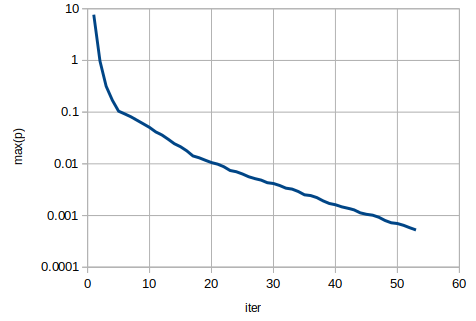
\includegraphics[width=0.6\linewidth]{linear2_simple_pres.png}
\end{center}


\subsubsection{Течение Пуазейля}
TODO

\subsubsection{Стационарное обтекание квадратного препятствия}

В тесте \ename{obstacle2-simple} из файла \ename{obstacle_2d_simple_test.cpp}
рассматривается задача о стационарном обтекании
квадтратного препятствия (см. постановку в п. \ref{sec:problem-obstacle}).
По окончании расчёта в консоль печатаются коэффициенты сопротивления и подъёмной силы.

Используется естественная нумерация узлов с неактивными ячейками.
Класс \cvar{RegularGrid2D} предлагает следующие методы, связанные с неактивными ячейками:
\begin{itemize}
\item
\cvar{void RegularGrid2D::deactivate_cells(Point bot_left, Point top_right)} -- установить область неактивных ячеек;
\item
\cvar{bool RegularGrid2D::is_active_cell(size_t icell)} -- проверить, является ли ячейка активной.
\end{itemize}

Кроме того, в задаче появились внутренние границы.
То есть для постаноки граничных условий уже не достаточно
использовать крайние значение индексов $i$, $j$,
а нужен механизм для получения граничных отрезков сетки.
Для этого введены следующие функции
\begin{itemize}
\item
\cvar{RegularGrid2d::boundary_yfaces()} -- получить список всех вертикальных граничных фасок (возвращает парные индексы в
соответствии \cvar{yface_centered_grid}.
\item
\cvar{RegularGrid2d::boundary_xfaces()}  -- получить список всех горизонтальных граничных фасок (возвращает парные индексы в
соответствии \cvar{xface_centered_grid}.
\item
\cvar{RegularGrid2d::yface_type(size_t yface_index)} -- узнать тип вертикальной грани по её глобальному индексу.
Возвращает перечисление
\begin{minted}[linenos=false]{c++}
enum struct FaceType{
	Internal,     // внутренняя
	Boundary,     // граничная
	Deactivated   // неактивная (находится внутри неактивной области)
};
\end{minted}
\item
\cvar{RegularGrid2d::xface_type(size_t xface_index)} -- узнать тип вертикальной грани по её глобальному индексу.
\end{itemize}

\subsubsubsection{Функция верхнего уровня}
\clisting{open}{"test/obstacle_2d_simple_test.cpp"}
\clisting{pass}{"TEST_CASE"}
Здесь сначала происходит установка параметров расчёта: числа Рейнольдса, параметра $E$,
количества итераций, порога сходимости и разбиения единичного интервала.
\clisting{lines-range}{"double Re", "n_unit"}
Далее строится сетка
\clisting{line}{"grid"}
В этом примере сетка строится в четырёхугольнике $[0, 12]\times[-2,2]$.
Потом для описания квадтратного препятствия 
происходит деактивация ячеек, находящихся в единичном квадрате
с нижней левой координатой $(2, -0.5)$ и верхней правой координатой $(3, 0.5)$.
\clisting{line}{"deactivate_cells"}
Потом создаётся решатель, инициализируются функции сохранения
и вызывается алгоритм потенциальной инициализации расчётных полей.
\clisting{until}{"worker.initialize();"}

Затем идёт стандартный цикл по SIMPLE-итерациям 
\clisting{block}{"size_t it = 0;"}

По окочании цикла вызывается функция сохранения решения в vtk
\clisting{line}{"worker.save_current_fields(it);"}

В конце происходит расчёт коэффициентов сил и их печать в консоль
\clisting{lines-range}{"coefs", "Cy"}
Результирующее поле течения сохраняется в файл \ename{obstacle2.vtk.series}.

\subsubsubsection{Учёт неактивных ячеек}
\clisting{to-start}{}
Неактивные ячейки учитываются во всех алгоритмах
сборки систем линейных уравнений. Рассмотрим на примере сборки
матрицы для пробной скорости, реализованной в функции \cvar{assemble_u_slae}.
\clisting{line}{"void Obstacle2DSimpleWorker::assemble_u_slae()"}
\clisting{pass}{"// internal"}
Рассмотрим цикл сборки внутренних узлов ``красной'' сетки для $u$
(или, что тоже самое, цикл по всем вертикальным граням основной сетки)
\clisting{lines-range}{"size_t j", "size_t i"}
Сначала вычисляется индекс строки (сквозной индекс текущей грани):
\clisting{line}{"row_index"}
Эта грань может быть либо внутренней, либо граничной (принадлежать внутренней вертикальной границе),
либо неактивной.
Выполняется проверка, является ли эта грань внутренней
\clisting{line}{"FaceType::Internal"}
Если да, то выполняется обычная процедура сборки
\clisting{before}{"else"}
Если нет (то есть грань либо неактивная, либо принадлежит внутренней границе),
то в диагональ ставится единица, в правую часть 0.
\clisting{block}{"else"}
Это отражает тот факт, что на внутренних границах $u=0$ из-за условий прилипания,
а для неактивных мы пишем тривиальное уравнение, просто чтобы матрица не была вырождена.

\clisting{to-start}{}
\clisting{pass}{"void Obstacle2DSimpleWorker::assemble_u_slae()"}
Учёт условий прилипания на внутренних горизонтальных
границах осуществляется через фиктивный узел в лямбда-функции \cvar{"add_to_mat"},
которая перехватывает все ситуации, когда алгоритм требует добавить что-либо в фиктивную колонку матрицы.
\clisting{line}{"auto add_to_mat"}
Такие ситуации могут произойти либо при сборке
около вертикальной грани, находящейся рядом с верхней границей:
\clisting{lines-range}{"if (ij_col[1] == _grid.ny())", "add_value"}
либо около вертикальной грани, находящейся рядом с нижней границей границей:
\clisting{lines-range}{"if (ij_col[1] == (size_t)-1)", "add_value"}
либо около вертикальнй грани, находящейся непосредственно над или под препятствием.
В этом случае индекс фиктивной колонки, в которую трубуется поставить будет
соответствовать неакотвной вертикальной грани.
Мы вычисляем этот индекс
\clisting{before}{"if"}
Если он неактивный, то следуем по процедуре добавления фиктивного узла около
границы с нулевым значением.
\clisting{block}{"if"}
Иначе -- это нормальная колонка и мы добавляем туда значение по стандартной процедуре
\clisting{line}{"add_value"}

\subsubsubsection{Расчёт коэффициентов сопротивления}
\label{sec:prog-cxcy}
\clisting{to-start}{}
Расчёт коэффициентов сил по формулам \cref{eq:ns2d_cx,eq:ns2d_cy} осуществляется в процедуре \cvar{coefficients()}.
Она возвращает структуру, куда входят все шесть искомых значений
\clisting{block}{"struct Coefficients"}
Процедура, объявленная как
\clisting{line}{"Obstacle2DSimpleWorker::coefficients()"}
производит вычисления четырёх интегралов по простой квадратуре
\cref{eq:ns2d_gamma_quadrature}.
Результаты аггрегируются в переменные
\clisting{lines-range}{"sum_cpx", "sum_cfy"}
Операции проводятся в циклах по внутренним граничным отрезкам.
Сначала рассматриваются вертикальные границы:
\clisting{line}{"for (const RegularGrid2D::split_index_t& yface: _grid.boundary_yfaces())"}
Здесь в переменную \cvar{yface} попадают все парные индексы вертикальных граней, лежащих
на границах. Сначала нужно отфильтровать границы, лежащие во входном и выходном сечениях
\clisting{until}{" else "}
На вертикальных границах актуально вычисление коэффициентов $C^p_x$, $C^f_y$ (из пункта \ref{sec:compute-obstacle-coefs}).
Дли их определения на каждой сеточной грани мы должны определить
$p\,n_x$, $\dsfr{v}{n}$ по формулах \cref{eq:ns2d_obstacle_dvdn_vertical,eq:ns2d_obstacle_pnx_vertical}.
\clisting{line}{"pnx"}
Для использования этих формул нужно определить, является ли это левой или правой границей обтекаемого тела.
Мы вычисляем индексы ячеек, лежащих слева и справа.
Если левая ячейка активна, значит это левая граница, если правая активна, значит это правая граница.
\clisting{until}{"right_cell"}
Далее левой границы
\clisting{lines-range}{"if", "dvdn"}
для правой
\clisting{lines-range}{"if", "dvdn"}
иначе (если это и не правая и не левая граница) бросается исключение,
потому что так быть не должно: у любой внутренней границы должна быть хоть одна соседняя активная ячейка
\clisting{block}{"else"}
После вычисления $p\,n_x$, $\dsfr{v}{n}$ они добавляются
в искомые интегралы согласно
\cref{eq:ns2d_gamma_quadrature}:
\clisting{lines-range}{"sum_cpx", "sum_cfy"}

Далее аналогичная процедура проводится для горизонтальных граней,
в результате которой вычисляются интегралы \cvar{sum_cpy}, \cvar{sum_cfx}.

\clisting{block}{"for (const RegularGrid2D::split_index_t& xface: _grid.boundary_xfaces())"}

В конце функции искомые коэффициенты вычисляются через
уже найденные интегралы согласно
\cref{eq:ns2d_cx,eq:ns2d_cy}:
\clisting{lines-range}{"Coefficients", "return"}

\subsubsubsection{Результаты расчёта}
Картина течения, полученная для
сетки \cvar{n_part = 10} при $\Ren = 20$,
представлена на \figref{fig:obstacle2-flow}
\begin{figure}[h!]
\centering
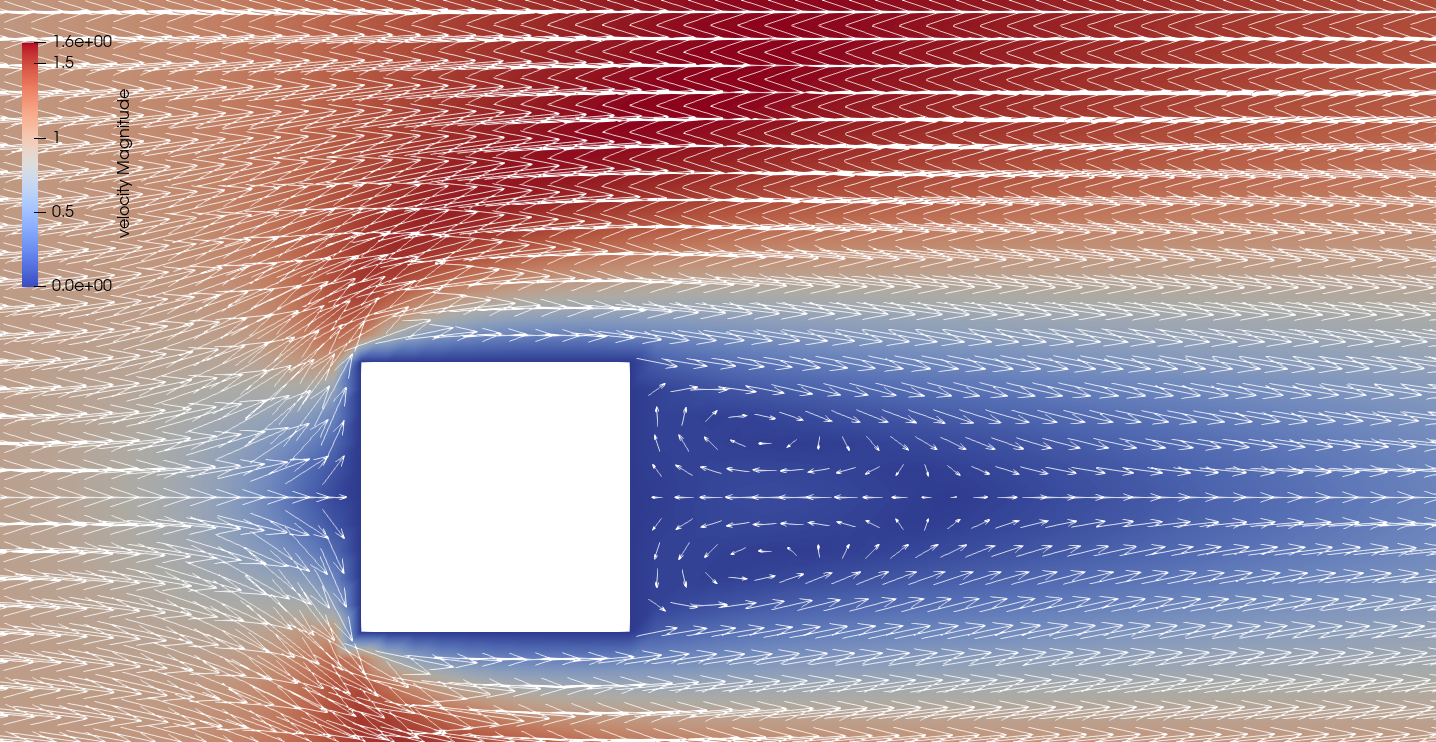
\includegraphics[width=0.9\linewidth]{obstacle2-flow.png}
\caption{Обтекание квадратного препятствия в стационарном режиме}
\label{fig:obstacle2-flow}
\end{figure}
Полученные коэффициенты сопротивления:
\begin{shelloutput}
=== Drag
Cpx = 2.97224
Cfx = 1.08639
Cx  = 4.05863
=== Lift
Cpy = -6.815e-10
Cfy = -1.64419e-10
Cy  = -8.45919e-10
\end{shelloutput}
Для $\eps = 10^{-1}$ решение сошлось за 29 итераций.

\subsubsection{Нестационарное обтекание квадратного препятствия с теплообменом}
\label{sec:prob-obstacle-temp}

Эта задача реализована в файле \ename{obstacle_nonstat_2d_simple_test.cpp}
в тесте \ename{[obstacle2-nonstat-simple]}.

Программа решает задачу в той же области, которая рассматривалась
в предыдущем пункте, но в нестационарной постановке
\cref{eq:ns2d_nonstat}
и с добавлением температуры
\cref{eq:ns2d_nonstat_temperature}.
Граничные условия для температуры имеют вид
\begin{align*}
(x,y)\in\Gamma_{in}:          \quad& T = 0, \\
(x,y)\in\gamma:               \quad& T = 1, \\
(x,y)\in\Gamma_{out,top,bot}: \quad& \dfr{T}{n} = 0.
\end{align*}

Поля течения для разных моментов времени пишутся в файл
\ename{obstacle-nonstat.vtk.series}. Кроме того, в файл \ename{c.txt}
пишутся вычисленные на разные моменты времени коэффициенты сопротивления и
интегральное число Нуссельта.

\subsubsubsection{Функция верхнего уровня}
\clisting{open}{"test/obstacle_nonstat_2d_simple_test.cpp"}
В начале обозначим параметры задачи:
числа Рейнольдса и Пекле,
разбиение единичного отрезка,
шаг по времени $\dt$ и конечное время, 
параметр внутреннего итерационного процесса $E$, 
максимальное количество итераций во внутреннем итерационном процессе
и порог по невязке:
\clisting{pass}{"TEST_CASE"}
\clisting{lines-range}{"Re", "eps"}

Далее проводится создание сетки (так же, как и в предыдущем примере) и начальная инициализация
решателя
\clisting{lines-range}{"grid", "save_current_fields"}

После всех инициализаций начинается цикл по времени
\clisting{line}{"for (double time=time_step; time<end_time+1e-6; time+=time_step)"}
Отметим, что поскольку значению $t=0$ соответствует начальное
состояние решения, то цикл начинается сразу с первого шага $t=\dt$.

Внутри цикла по времени производится цикл
внутренних итераций SIMPLE
\clisting{block}{"size_t it"}

Далее, если текущее время кратно $1.0$, производится сохранение
решения в файл vtk и запись коэффициентов сил в файл:
\clisting{block}{"if"}

Печатается информация о сходимости текущей итерации
\clisting{line}{"cout"}

и производится переход на следующий шаг по времени:
\clisting{line}{"to_next_time_step"}

\subsubsubsection{Учёт нестационарности}
Согласно пунку \ref{sec:ns2d-nonstat} наличие производной по времени
учитывается:
\begin{itemize}
\item
При вычислении коэффициентов $d^u$, $d^v$
\cref{eq:ns2d_nonstat_duv}:
\clisting{to-start}{}
\clisting{pass}{"ObstacleNonstat2DSimpleWorker::ObstacleNonstat2DSimpleWorker("}
\clisting{lines-range}{"_du", "_dv"}
\item
При сборке систем уравнений для $u^*$, $u^*$
\cref{eq:ns2d_nonstat_uvstar}
\clisting{to-start}{}
\clisting{pass}{"void ObstacleNonstat2DSimpleWorker::assemble_u_slae()"}
как прибавка к диагонали
\clisting{line}{"add_to_mat(row_index, {i, j}, 1.0 + _tau/_time_step)"}
и правой части
\clisting{line}{"_rhs_u[row_index] += (_tau/_time_step)*_u_old[row_index]"}
\item
А так же в граничных условиях на выходе.
В этом случае условия \cref{eq:ns2d_outflow_common}
для $u$ по аналогии с \cref{eq:ns2d_outflow_common_semi}
аппроксимируются к виду
\begin{equation*}
(x,y)\in\Gamma_{out}:\; \frac{\hat u - \check u}{\dt} + \frac{\hat u - u}{\tau} + u\dfr{\hat u}{x} = 0.
\end{equation*}
Для упрощения по прежнему будем использовать ``стационарное'' условие
для поперечной скорости $v=0$.
Тогда для $u^*$ можно записать
$$
(x,y)\in\Gamma_{out}:\;
	\left(1 + \frac{\tau}{\dt}\right)u^*_{n_x, j+\tfrac12}
	+ \tau U_{n_x, j+\tfrac12}\frac{u^*_{n_x, j+\tfrac12}
	                                - u^*_{n_x-1, j+\tfrac12}}{h_x}
	= u_{n_x, j+\tfrac12}
        + \frac\tau\dt \check u_{n_x, j+\tfrac12}
$$
Это выражение и добавляется в соответствующие строки матрицы и правой части
\clisting{to-start}{}
\clisting{pass}{"void ObstacleNonstat2DSimpleWorker::assemble_u_slae()"}
\clisting{block}{"// right boundary: du/dt + u*du/dx = 0"}
\item
При переходе на слудующий шаг по времени в функции
\clisting{to-start}{}
происходит вычисление текущего значения температуры, и
присваивание значений $\check u$, $\check v$.
\clisting{block}{"double ObstacleNonstat2DSimpleWorker::to_next_time_step()"}
Вызов \cvar{set_uvp} здесь осуществляется для пересборки актуальных матриц.

\end{itemize}

\subsubsubsection{Расчёт температурного поля}
Осуществляется в функции
\clisting{to-start}{}
\clisting{line}{"ObstacleNonstat2DSimpleWorker::compute_temperature()"}
Для сборки системы
используется цикл по ячейкам сетки
\clisting{block}{"for (size_t j=0; j < _grid.ny(); ++j)"}
для активных ячеек используются формулы
\cref{eq:ns2d_nonstat_temperature_scheme},
а для неактивных -- тривиальное уравнение $T=0$.

Учёт граничных условий осуществляется за счёт фиктивных узлов
в функции \cref{add_to_mat}
\clisting{to-start}{}
\clisting{pass}{"ObstacleNonstat2DSimpleWorker::compute_temperature()"}
\clisting{line}{"add_to_mat"}

Для левой границы условия первого рода
\cref{eq:ns2d_temperature_bc1_scheme} с $T^\Gamma = 0$
\clisting{lines-range}{"left boundary", "add_value"}
для нижней, верхней и выходной -- 
условия второго рода с $q=0$ \cref{eq:ns2d_temperature_bc2_scheme}:
\clisting{lines-range}{"right boundary", "add_value"}
Для границы обтекаемого тела -- условия первого рода
\cref{eq:ns2d_temperature_bc1_scheme} с $T^\Gamma = 1$:
\clisting{lines-range}{"internal boundary", "rhs"}

После сборки правой и левой частей происходит
решение СЛАУ и возвращается ответ
\clisting{lines-range}{"temperature", "return"}

\subsubsubsection{Вычисление коэффициента теплообмена}
Производится в той же функции, где и другие коэффициенты (см. п.\ref{sec:prog-cxcy})
\clisting{to-start}{}
\clisting{line}{"ObstacleNonstat2DSimpleWorker::coefficients()"}
В цикле по вертикальным границам
\clisting{line}{"_grid.boundary_yfaces()"}
на левой границе обтекаемого тела согласно формуле
\cref{eq:dtdn_scheme} имеем
\clisting{line}{"nu ="}
Здесь \cvar{left_cell} -- индекс ячейки, лежащей слева от рассматриваемого участка границы,
а $T^\Gamma = 1$ -- значение температуры из граничного условия.
Аналогичные выражения исользованы для правых
\clisting{line}{"nu ="}
нижних
\clisting{line}{"nu ="}
и верхних фасок
\clisting{line}{"nu ="}

После определения нормальной производной по температуре
она добавляется в интеграл согласно \cref{eq:ns2d_gamma_quadrature}.
Например, для горизонтальных границ
\clisting{line}{"sum_nu +="}

\subsubsubsection{Результаты расчёта}

\begin{figure}[h!]
\centering
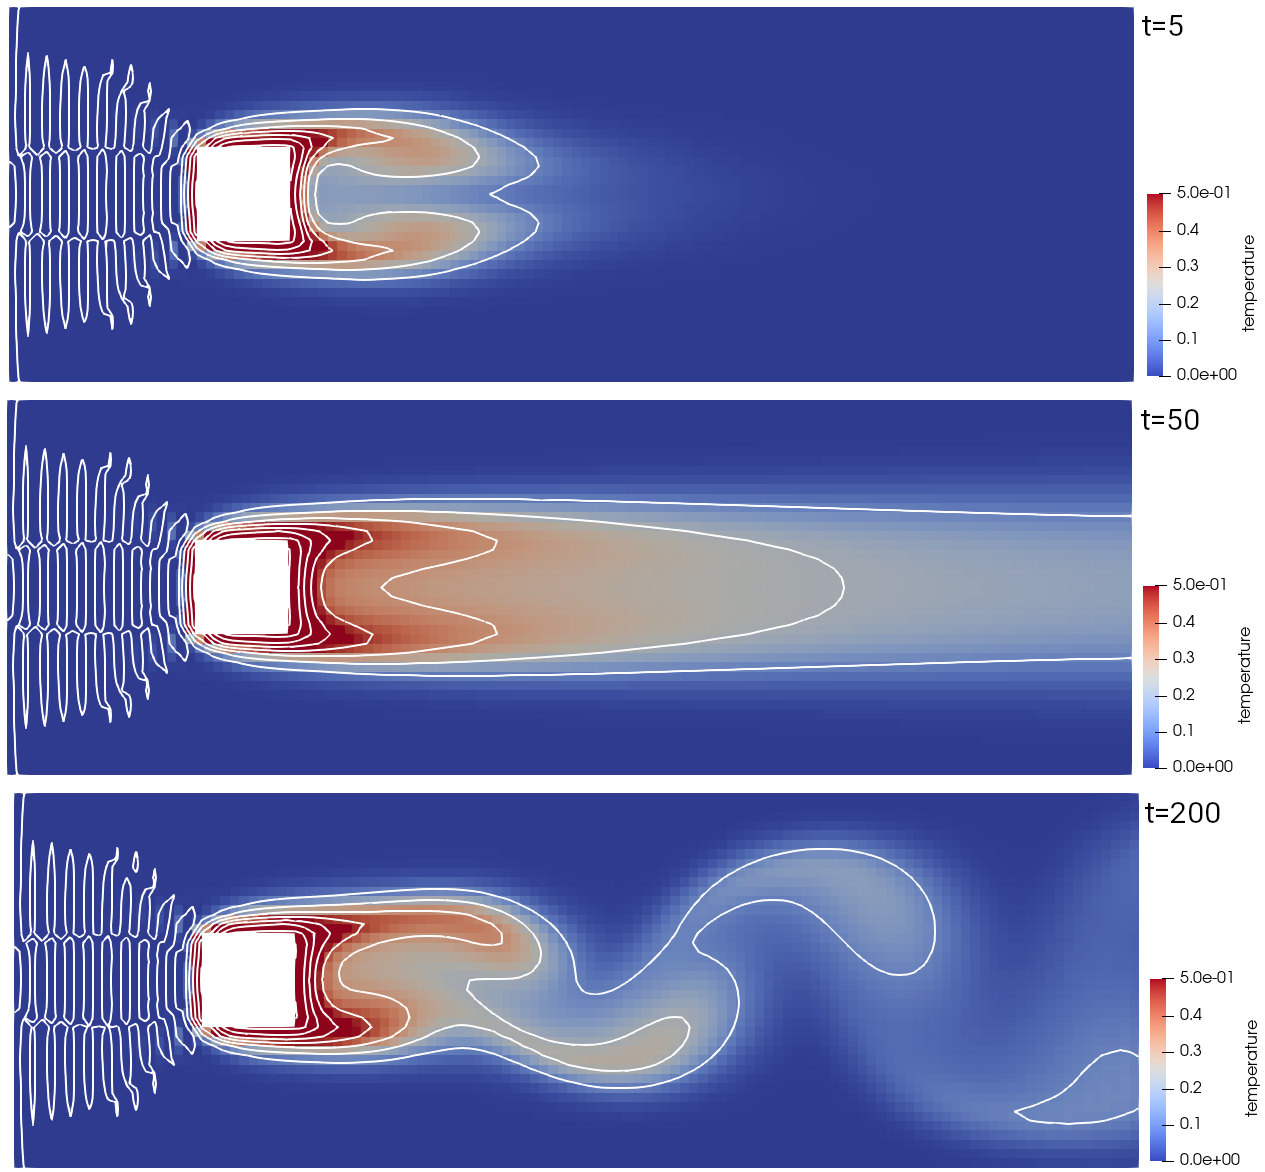
\includegraphics[width=1.0\linewidth]{temperature-obstacle2-simple.png}
\caption{Температурное поле при решении нестационарной задачи обтекания. Моменты времени $t=5$, $t=50$, $t=200$}
\label{fig:temperature-obstacle2-simple}
\end{figure}

Настояющую задачу будем решать с параметрами
$\Ren = 100$, $\Pen = 100$, $\eps=10^{-1}$, $\dt = 0.1$, $t_{end} = 200$, $n=10$.

На \figref{fig:temperature-obstacle2-simple}
представлено поле температуры на разные моменты времени.
Видно, что сначала нагреваемая жидкость продвигается вниз по потоку,
потом, на момент времени $t\approx50$ поток устанавливается,
но, в районе $t\approx100$ решение теряет устойчивость
и за препятствием образуется дорожка Кармана.

На \figref{fig:temperature-obstacle2-simple-iters}
представлено зависимость количество проведённых итераций
от времени. На начальном этапе, пока течение
развивается от состояния потенциального обтекания (начальное условие),
количество итераций велико, затем, с достижением решения
локального установления, решение начинает сходится за одну итерацию.
Но после $t>100$, когда начинает развиваться неустойчивость, количество
итераций вновь возрастает. Количество итераций на слое характеризует
степень изменения решения при продвижении к следующему шагу по времени.

\begin{figure}[h!]
\centering
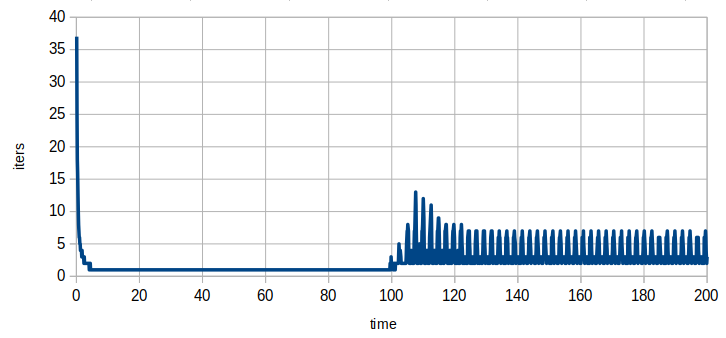
\includegraphics[width=0.8\linewidth]{temperature-obstacle2-simple-iters.png}
\caption{Зависимость количества внутренних итераций SIMPLE от момента времени}
\label{fig:temperature-obstacle2-simple-iters}
\end{figure}

Коэффициенты сопротивления, подъёмной силы и теплоотдачи нарисованы на \figref{fig:temperature-obstacle2-simple-coefs}.
Переход к нестационарному режиму течения характеризуется повышением теплоотдачи и сопротивлению
и появлению заметных осцилляций в подъёмной силе.

\begin{figure}[h!]
\centering
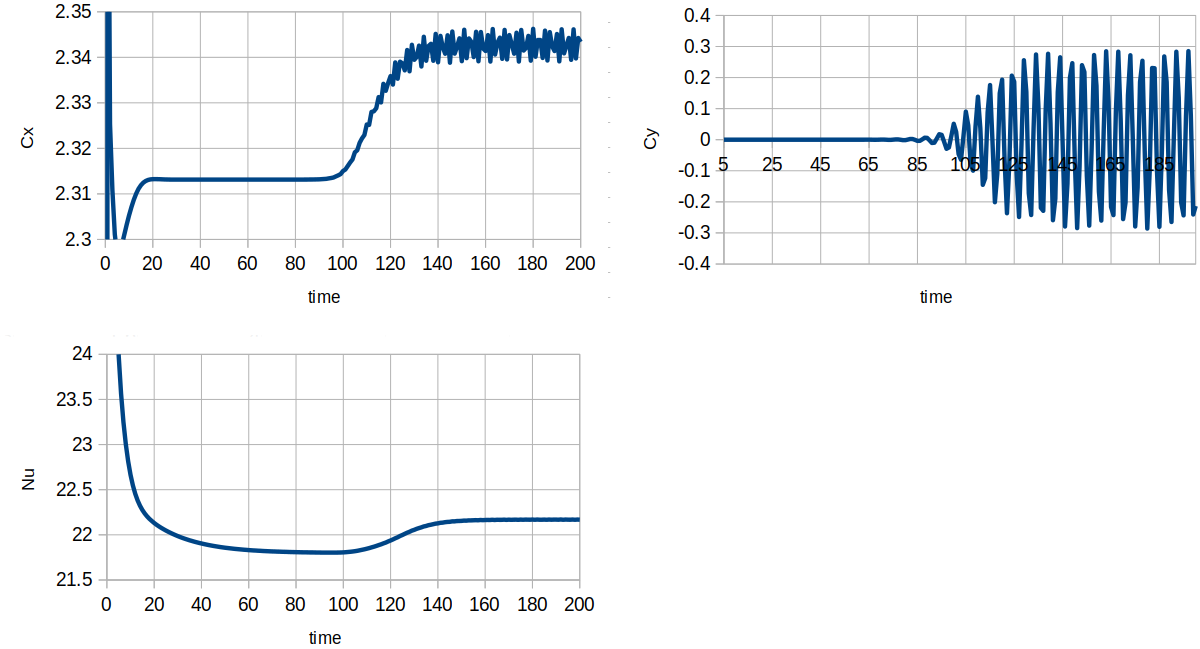
\includegraphics[width=1.0\linewidth]{temperature-obstacle2-simple-coefs.png}
\caption{Эволюция коэффициентов сопротивления $C_x$, подъёмной силы $C_y$ и теплоотдачи $\Nun$}
\label{fig:temperature-obstacle2-simple-coefs}
\end{figure}

Следует обратить внимание на небольшую рябь в поле температур, заметную
слева от препятствия на \figref{fig:temperature-obstacle2-simple}.
Её хорошо видно на трёхмерном отображении (см. \figref{fig:temperature-obstacle2-simple-temp3d}).
Если обратить внимаение на легенду, то можно заметить, что температура в этой
области даже становится отрицаетельной, что физически невозможно в рамках поставленных граничных условий.

Причина этой ряби кроется в симметричной разности, которую мы использовали
для аппроксимации конвективного слагаемого уравнения температуры (см. \cref{eq:ns2d_temperature_bc1_scheme}).
Известно, что симметричные разности склонны давать осциллирующее решение (даже если оно и устойчиво).
Если бы мы использовали схему против потока, то этой нефизичности в решении бы не было,
но при этом решение бы имело первый порядок точности по пространству.


\begin{figure}[h!]
\centering
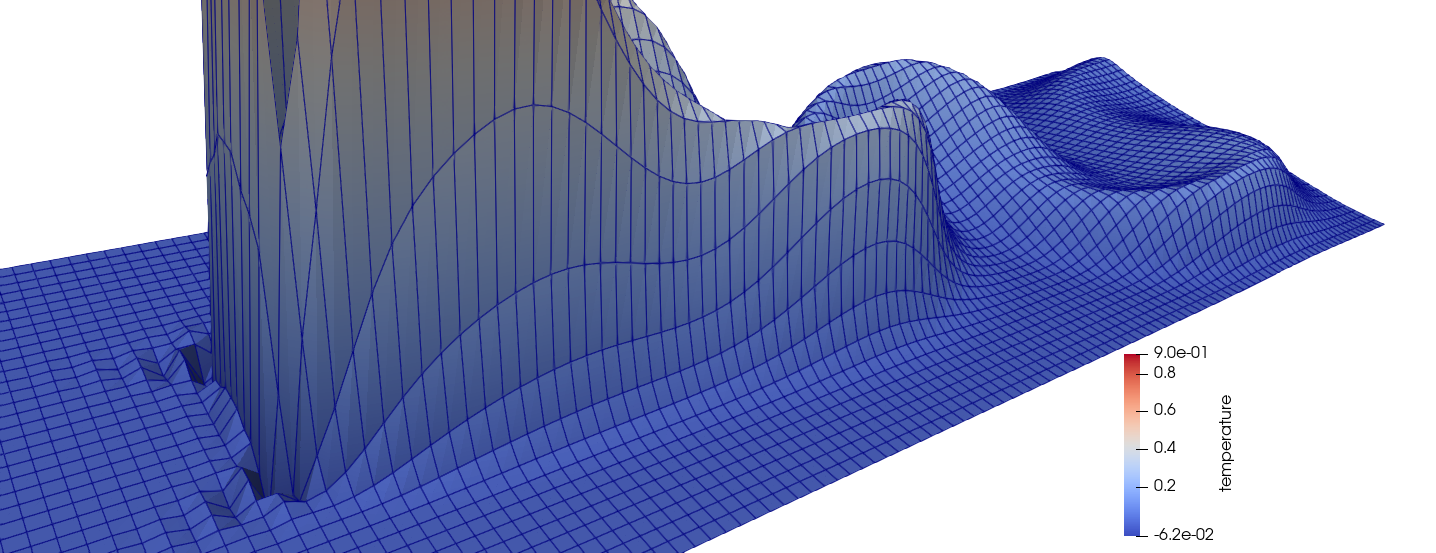
\includegraphics[width=1.0\linewidth]{temperature-obstacle2-simple-temp3d.png}
\caption{Температура на момент $t=150$ в трёхмерном отображении. Нефизичные осцилляции в области перед препятствием}
\label{fig:temperature-obstacle2-simple-temp3d}
\end{figure}


\subsection{Задание для самостоятельной работы}
Решить задачу с двумя обтекаемыми телами: одно расположено
в прямоугольнике
$$
\gamma_1: \begin{cases}
2.0 \leq x \leq 2.5, \\
-0.7 \leq y \leq 0.3,
\end{cases}
$$
второе --
$$
\gamma_2: \begin{cases}
4 \leq x \leq 4.5, \\
-0.3 \leq y \leq 0.7.
\end{cases}
$$

Использовать условия для температуры:
\begin{align*}
(x, y) \in \gamma_1: \quad T=0.5,\\
(x, y) \in \gamma_2: \quad T=1.0.
\end{align*}

Область расчёта и остальные граничные условия использовать те же, что и
в рассмотренной в п. \ref{sec:prob-obstacle-temp} задаче.
Параметры задачи:
$\Ren = 100$, $\Pen = 100$, $\eps=10^{-1}$, $\dt = 0.1$, $t_{end} = 200$, $n=10$.

Подсчитать коэффициенты сопротивления и теплоотдачи для каждого из двух
тел в отдельности. Нарисовать графики из изменения со временем.

Делать на основе программы из файла \ename{obstacle_nonstat_2d_simple_test.cpp}.

\paragraph{Задание сетки с неактивными ячейками}
\clisting{to-start}{}
\clisting{pass}{"TEST_CASE"}
Обтекаемые препятствия следует задавать
при определении сетки
\clisting{line}{"deactivate_cells"}
указав там по очереди две нужные области.

\paragraph{Задание граничных условий на температуру}
Поскольку в задаче граничные условия на обтекаемых
телах отличаются по своему значению, то следует
модифицировать алгоритм их задания.
Граничные условия на температуру задаются в функции \cvar{compute_temperature}
в строке
\clisting{to-start}{}
\clisting{pass}{"ObstacleNonstat2DSimpleWorker::compute_temperature()"}
\clisting{lines-range}{"internal boundary", "rhs"}

Согласно форме
\cref{eq:ns2d_temperature_bc1_scheme}
изменения в левой части не зависит от величины граничной температуры,
а в провой -- пропорционально ей.
Таким образом, для первого тела (где $T^\Gamma = 0.5$) добавка в правую часть будет иметь вид
\begin{minted}[linenos=false]{c++}
rhs[row_index] -= 2*value*0.5,
\end{minted}
а для второго -- останется такой же.

При этом нужно уметь отличать грани \cvar{row_index}, принадлежащие
первому телу от граней, принадлежащих второму.
Для этого в классе \cvar{ObstacleNonstat2DSimpleWorker} можно
объявить функцию, которая определяет ближайшую к ячейке границу.
Саму функцию можно реализовать просто используя координаты
центра ячейки \cvar{_grid.cell_center(icell)}. Например:
\begin{minted}[linenos=false]{c++}
// => 1 если ячейка icell близка к первому обтекаемому телу и 2 - если ко второму
int ObstacleNonstat2DSimpleWorker::gamma_closest_to_cell(size_t icell){
	double x = _grid.cell_center(icell).x();
	if (x < 3.25) {  // центр между первым и вторым телами
		return 1;
	} else {
		return 2;
	}
}
\end{minted}
Тогда можно написать
\begin{minted}[linenos=false]{c++}
double t_gamma;
if (gamma_closest_to_cell(row_index) == 1){
	t_gamma = 1.0;
} else {
	t_gamma = 0.5;
}
rhs[row_index] -= 2*t_gamme*value;
\end{minted}

\paragraph{Вычисление коэффициентов}
Во-первых следует модифицировать структуру, хранящую коэффициенты,
сделав там отдельные записи для каждого тела:
\begin{minted}[linenos=false]{c++}
struct Coefficients{
	double cpx1, cpx2;
	double cpy1, cpy2;
	double cfx1, cfx2;
	double cfy1, cfy2;
	double cx1, cx2;
	double cy1, cy2;
	double dtdn1, dtdn2;
};
\end{minted}
Во-вторых в функции сохранения этих коэффициентов в файл
в функции \cref{ObstacleNonstat2DSimpleWorker::save_current_fields}
\begin{minted}[linenos=false]{c++}
cx_writer << time << " ";
cx_writer << coefs.cx1 << " " << coefs.cy1 << " " << coefs.dtdn1 << " ";
cx_writer << coefs.cx2 << " " << coefs.cy2 << " " << coefs.dtdn2 << " ";
\end{minted}
Соответственно можно поправить легенду в функции \cref{initialize_saver}.

Сами коэффициенты следует вычислять в функции \cref{coefficients()}.
Там нужно завести аггрегаторы на оба тела:
\begin{minted}[linenos=false]{c++}
double sum_cpx1 = 0;
double sum_cpy1 = 0;
double sum_cfx1 = 0;
double sum_cfy1 = 0;
double sum_nu1  = 0;
double sum_cpx2 = 0;
double sum_cpy2 = 0;
double sum_cfx2 = 0;
double sum_cfy2 = 0;
double sum_nu2  = 0;
\end{minted}

И далее заполнять их в зависимости от близости ячейки. Например для вертикальных граней
\begin{minted}[linenos=false]{c++}
if (gamma_closest_to_cell(left_cell) == 1){
	sum_cpx1 += pnx * _hy;
	sum_cfy1 += dvdn * _hy;
	sum_nu1 += nu * _hy;
} else {
	sum_cpx2 += pnx * _hy;
	sum_cfy2 += dvdn * _hy;
	sum_nu2 += nu * _hy;
}
\end{minted}

В конце нужно правильным образом заполнить все поля
переменной \cvar{coef}.
\begin{minted}[linenos=false]{c++}
	coefs.cpx1 = 2.0*sum_cpx1;
	coefs.cpx2 = 2.0*sum_cpx2;
	...
\end{minted}
